%
%

\documentclass[a4paper,11pt]{article}
\pdfoutput=1 

\usepackage{jinstpub} 

\usepackage{lineno}
%\linenumbers

\usepackage{enumerate}

\title{\boldmath An analytical model for photomultiplier tube calibration}

\author[a]{L. N. Kalousis}
\affiliation[a]{Physics Department, National Technical University, 157 80 Zografou, Athens, Greece}
\emailAdd{leonidas.kalousis@gmail.com}

\abstract{The purpose of the present publication is to offer an analytical model that can be used for the calibration of photomultiplier tubes (PMTs). 
The derivation of the mathematical formulae involved is discussed extensively and we apply this machinery to a real problem; the gain determination of the R7081 Hamamatsu PMT. 
 We hope that our work can provide a third, powerful alternative to the task of gain deconvolution. 
 We also believe that the techniques explained in this article can be applied to other problems in PMT calibration and monitoring. }

\keywords{Photon detectors for UV, visible and IR photons (vacuum) (photomultipliers, HPDs, others); 
Detector alignment and calibration methods (lasers, sources, particle-beams);
Analysis and statistical methods; 
Data analysis}

\arxivnumber{2304.08735} 

\begin{document}
\maketitle
\flushbottom

\section{Introduction}
\label{sec:intro}
% 

The standard machinery for photomultiplier tube (PMT) calibration has been presented in an influential paper written by E. H. Bellamy and collaborators, ref.~\cite{bellamy}. 
Years later, R. Dossi \emph{et al.} proposed a specific model for the single photoelectron (SPE) response function that can treat a vast number of PMTs. 
It was based on a carefully chosen combination of an exponential and a truncated gaussian distribution, ref.~\cite{dossi}:
\begin{align}
S(x) =    \left( \ w \alpha e^{-\alpha x } + (1-w)\frac{1}{g_N} \frac{1}{\sqrt{2\pi}\sigma} e^{ - \frac{( x - Q )^2}{2\sigma^2}} \ \right) H(x).       \label{eq:S}
\end{align}
The mathematical formulae involved in the Dossi model are rather complicated and an analytical solution has eluded experimental physicists. 
Up to now, two main approaches are available for the deduction of the charge response function $S_R(x)$.
\begin{enumerate}[i.]
\item  A method that computes the convolution integrals numerically, using a recursive algorithm, 
for the the first photoelectron (PE) peaks and approximates higher order corrections with symmetric gaussians~\cite{dossi,darkside}. 
\item A novel technique, based on the Discrete Fourier Transform (DFT), that calculates the charge response function $S_R(x)$ numerically for all orders in the Poisson mean $\mu$~\cite{me2}. 
\end{enumerate}
Both procedures give consistent results when carefully applied. 
In this article, we have tried to solve the Dossi model analytically offering thus a third solution to this task. 
Therefore, no new results are obtained. Nonetheless, it is always a rare pleasure to discover new solutions to old riddles. 
Moreover, we hope that this new approach can provide answers to problems where the aforementioned methods fail for one reason or the other. 

The paper is organized as follows. 
In section~\ref{sec:mod} we present in great detail the calculations that lead to the analytical model we put forward. 
It should be emphasized from the onset that, while the mathematics might seem unnecessary and elaborate at first glance, the final equations are rather simple and easy to implement. 
In section~\ref{sec:res} we apply this formula to the calibration of the Hamamatsu R7081 PMT. 
Attention was paid to showcase that the analytical model provides consistent figures with the already established methods. 
We close this publication with some general remarks concerning further uses of this mathematical scheme. 


\section{Analytical model}
\label{sec:mod}
%

\subsection{General form of $S^{(n)}_R(x)$ }
%

The charge response of a PMT, when illuminated with light pulses of constant number of photons, is dictated by the function $S_R(x)$:
\begin{align}
S_R(x) = \sum_{n=0}^{+\infty} P(n;\mu) S^{(n)}_R(x),
\end{align}
where 
\begin{align}
S^{(n)}_R(x) = (S_n*B)(x). 
\end{align}
$ P(n;\mu)$ is the Poisson distribution with mean value $\mu$. 
$S_n(x)$ corresponds to the $n$-times convolution of the SPE response function $S(x)$ and $B(x)$ refers to the pedestal. 
An extensive review describing the main steps in PMT calibration can be found elsewhere~\cite{me2}. 
Let us assume, following the paper of Dossi \emph{et~al.}, that the SPE charge amplification can be written as:
\begin{align}
S(x) = w f(x) + (1-w)g(x),
\end{align}
where 
\begin{align}
f(x) = \alpha e^{-\alpha x } \ H(x),
\end{align}
and
\begin{align}
g(x) = \frac{1}{g_N} \frac{1}{\sqrt{2\pi}\sigma} \ e^{ - \frac{( x - Q )^2}{2\sigma^2}} \ H(x). 
\end{align}
The principal $S^{(n)}_R(x)$ functions can then be written as:
\begin{align}
S^{(n)}_R(x) & = \sum_{m=0}^{n}  \frac{n!}{m!(n-m)!} \ w^m (1-w)^{n-m} (f_m*g_{n-m} *B )(x)\nonumber \\
                     & = (1-w)^n (g_{n} *B )(x) + \sum_{m=1}^{n}  \frac{n!}{m!(n-m)!} \ w^m (1-w)^{n-m} (f_m*g_{m-n} *B )(x), \label{eq:snr1}
\end{align}
where the $f_m(x)$ and $g_{n-m}(x)$ are the $m$-times and $(n-m)$-times convolutions of $f(x)$ and $g(x)$ respectively. 
In this last step we made use of the binomial expansion for $S_n(x)$ \cite{binom}. 
The formula can be simplified by setting:
\begin{align}
G_n(x) = (g_{n} *B )(x), 
\end{align}
and 
\begin{align}
h_{m,n}(x) = (f_{m} * G_{n-m} )(x).  
\end{align}
Like this eq.~\eqref{eq:snr1} can be expressed as:
\begin{align}
S^{(n)}_R(x) & = (1-w)^n G_n(x) + \sum_{m=1}^{n}  \frac{n!}{m!(n-m)!} \ w^m (1-w)^{n-m} h_{m,n}(x). \label{eq:snr2}
\end{align}
We proceed to calculate each term in eq.~\eqref{eq:snr2} separately.  


\subsection{Calculation of $S^{(0)}_R(x)$ and $S^{(1)}_R(x)$}
%

The zeroth term of $S^{(n)}_R(x)$ can be computed easily. 
The result is:
\begin{align}
S^{(0)}_R(x)  = \ & B(x) \nonumber \\
                      = \ & \frac{1}{\sqrt{2\pi}\sigma_0} \ e^{-\frac{(x-Q_0)^2}{2\sigma_0^2}}.
\end{align}
We remind the reader that $f_0(x)=g_0(x)=\delta (x)$. 
This is the well-known pedestal distribution and $Q_0$ and $\sigma_0$ are the mean value and standard deviation of $B(x)$ respectively. 
On the other hand, the $n=1$ term recieves two contributions:
\begin{align}
S^{(1)}_R(x)  = w (f*B)(x) + (1-w)(g*B)(x). 
\end{align}                     
We begin with the formula of $(f*B)(x)$ and we then write down $(g*B)(x)$.

The convolution between $f(x)$ and $B(x)$ is given by the equation:
\begin{align}
(f*B)(x)  = \ \frac{\alpha}{2} e^{\frac{\alpha^2\sigma_0^2}{2}} e^{-\alpha (x-Q_0)} \ \text{erfc}\left( \frac{Q_0 + \alpha\sigma_0^2 - x }{\sqrt{2}\sigma_0} \right),
\end{align}  
where erfc is the complementary error function~\cite{erf}.
On the other hand, $(g*B)(x)$ equals to:
\begin{align}
(g*B)(x)  = \ \frac{1}{2} \frac{1}{g_N} \frac{1}{\sqrt{2\pi}} \frac{1}{\sqrt{\sigma_0^2 + \sigma^2}} \ e^{ -\frac{ (x-Q_0-Q)^2 }{2(\sigma_0^2 + \sigma^2)}} 
\ \text{erfc}\left(  \frac{ Q_0\sigma^2 -Q\sigma_0^2 -x \sigma^2  }{\sqrt{2} \sigma_0\sigma\sqrt{\sigma_0^2 + \sigma^2} }   \right).
\end{align}  
The proof of both these formulae is challenging and interesting in its own right and it is presented in the appendix~\ref{app:sr1} with great care. 

\subsection{Gaussian approximation of $G_n(x)$}
%

A direct calculation of $G_n(x)$, 
\begin{align}
G_n(x)  = (g_n*B)(x),
\end{align}   
for $n\geq 2$ appears to be both difficult and complicated. 
Perhaps the mathematics can be worked out in some systematic way, but the resulting equations ought to be elaborate to be implemented efficiently in an analysis software. 
For the reasons above, we took the decision to approximate all truncated gaussians in $G_n(x)$ with perfectly symmetric ones. 
In this way $G_n(x)$ becomes:
\begin{align}
G_n(x)  = \ \frac{1}{\sqrt{2\pi} \sigma_n } \ e^{ -\frac{ (x-Q_n)^2 }{2\sigma_n^2} },
\end{align}   
where
\begin{align}
Q_n  = Q_0 + n Q_g, \\
\sigma_n^2 = \sigma_0^2 + n \sigma_g^2.  
\end{align}   
Since several convolutions are involved, the truncation of $g(x)$ at negative values of charge should have little impact on the final result.  
$Q_g$ and $\sigma_g$ are the mean value and standard deviation of $g(x)$ and their exact formulae can be found in ref.~\cite{me}.


\subsection{$h_{m,n}(x)$ in terms of hypergeometric functions}
%

The major difficulty we faced in trying to solve the analytical model, lied in the calculation of $h_{m,n}(x)$. 
As the reader can verify the final solution involves the use of special functions and it is far from trivial. 
The answer is:
\begin{align}
h_{m,n}(x) =  \frac{\alpha (\alpha\sqrt{2} \sigma_{n-m})^{m-1}}{(m-1)!} \frac{1}{2\sqrt{\pi}} \  I_{m,n}.
\end{align}  
%where 
%\begin{align}
%\sigma^2_{m,n} = \sigma^2_0 + (n-m)\sigma^2_g.
%\end{align}  
The expression for $I_{n,m}$ turns out to be:
\begin{align}
I_{m,n} = 
\begin{cases}
2\sqrt{\pi}   e^{\omega^2 - \psi^2 + (m-1) \ell n |\omega|},  & \omega>0 \ \text{and} \  \omega^2 \gg 0\\
e^{\omega^2 -\psi^2 } \left(\  \Gamma\left( \frac{m}{2} \right) M\left(-\frac{m-1}{2}, \frac{1}{2}, -\omega^2 \right)  
+ 2|\omega| \Gamma\left( \frac{m+1}{2} \right) M\left(1-\frac{m}{2}, \frac{3}{2}, -\omega^2 \right)   \    \right), &  \omega > 0  \\
e^{ -\psi^2 } \Gamma\left( \frac{m}{2} \right)   \Gamma\left( \frac{m+1}{2} \right) \frac{1}{\sqrt{\pi}} U\left( \frac{m}{2}, \frac{1}{2}, \omega^2  \right), & \omega<0
\end{cases}
\nonumber
\end{align} 
where $M(a,b,z)$ and $U(a,b,z)$ are the \emph{confluent hypergeometric functions} of the first and second kind respectively. 
The derivation can be found in the appendix~\ref{app:Imn}. 
The variables $\omega$ and $\psi$ are given by the relations:
\begin{align}
\psi = & \frac{x-Q_{n-m}}{\sqrt{2}\sigma_{n-m}}, \\
\omega = & \frac{x-Q_{n-m} -\lambda\sigma^2_{n-m}}{\sqrt{2}\sigma_{n-m}}.
\end{align}  
%and
%\begin{align}
%Q_{m,n} = Q_0 + (n-m)Q_g. 
%\end{align}  
%In our case the constant $c$ was set to twenty and that was enough for our investigations. 
Note that an asymptotic formula can be applied to $U(a,b,c)$ as well, for $\omega < 0$ and $\omega^2 \gg 0$, but this was not necessary in our work. 
Note also that for large $n$ the $h_{m,n}(x)$ functions can be approximated by symmetric gaussians to simplify the equations but, again, this was not done in this study. 


\section{Calibration of the Hamamatsu R7081 photomultiplier}
\label{sec:res}
%

Several data sets were taken with a Hamamatsu R7081 PMT. 
The details of the experimental setup have been described before in ref.~\cite{me2} and will not be repeated here. 
In a nutshell, the R7081 PMT was placed inside a dark, light-tight box. Light pulses were created by a light emitting diode (LED) connected to a fast pulse generator. 
The photons were carried inside the box through an optical fiber and the signals from the PMT were readout by a LeCroy WavePro 725Zi oscilloscope.   
The setup triggered on the generator's second, duplicated channel and all signals were recorded. Including those with no photons at all (pedestal). 

\begin{figure}[!t]
\centering
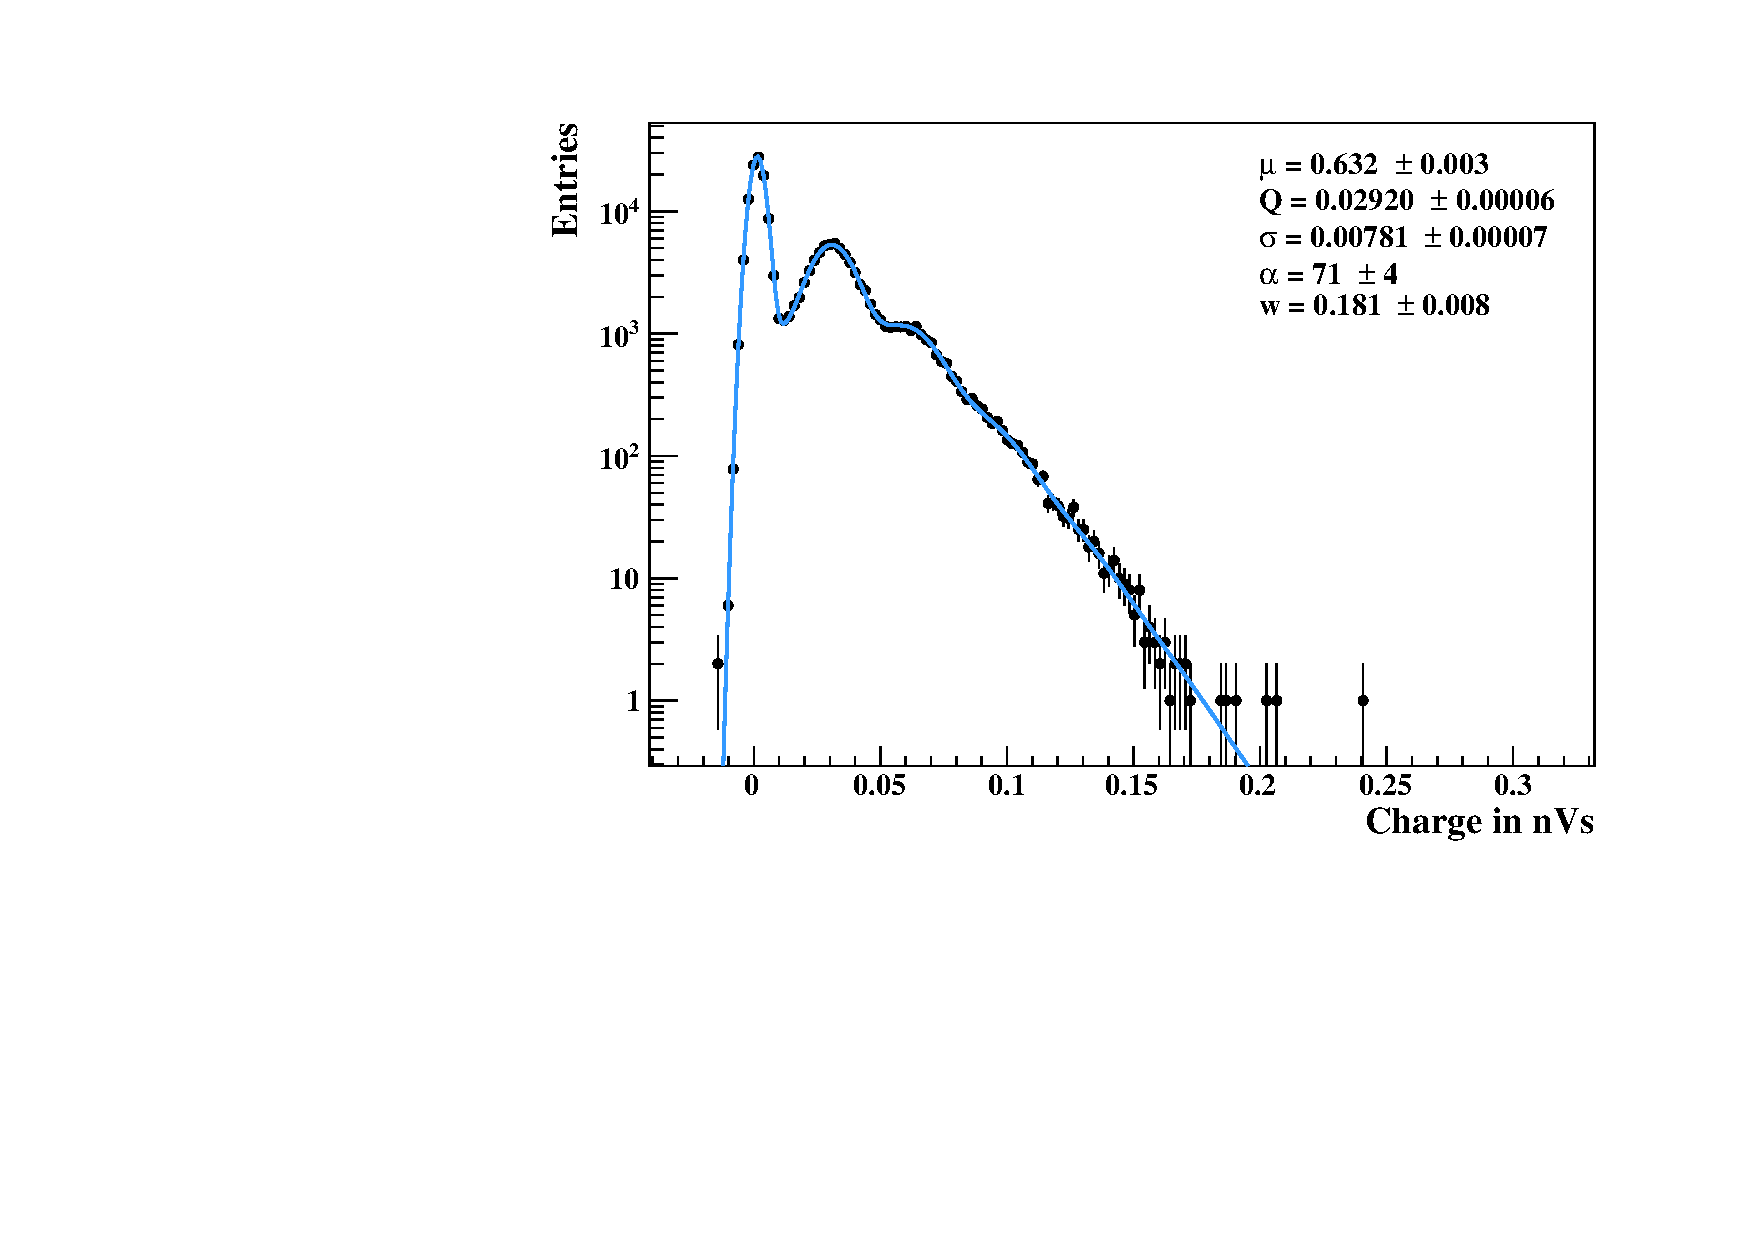
\includegraphics[width=11.3cm, height=7.8cm]{figures/fit-1.pdf} \\[1.5ex]
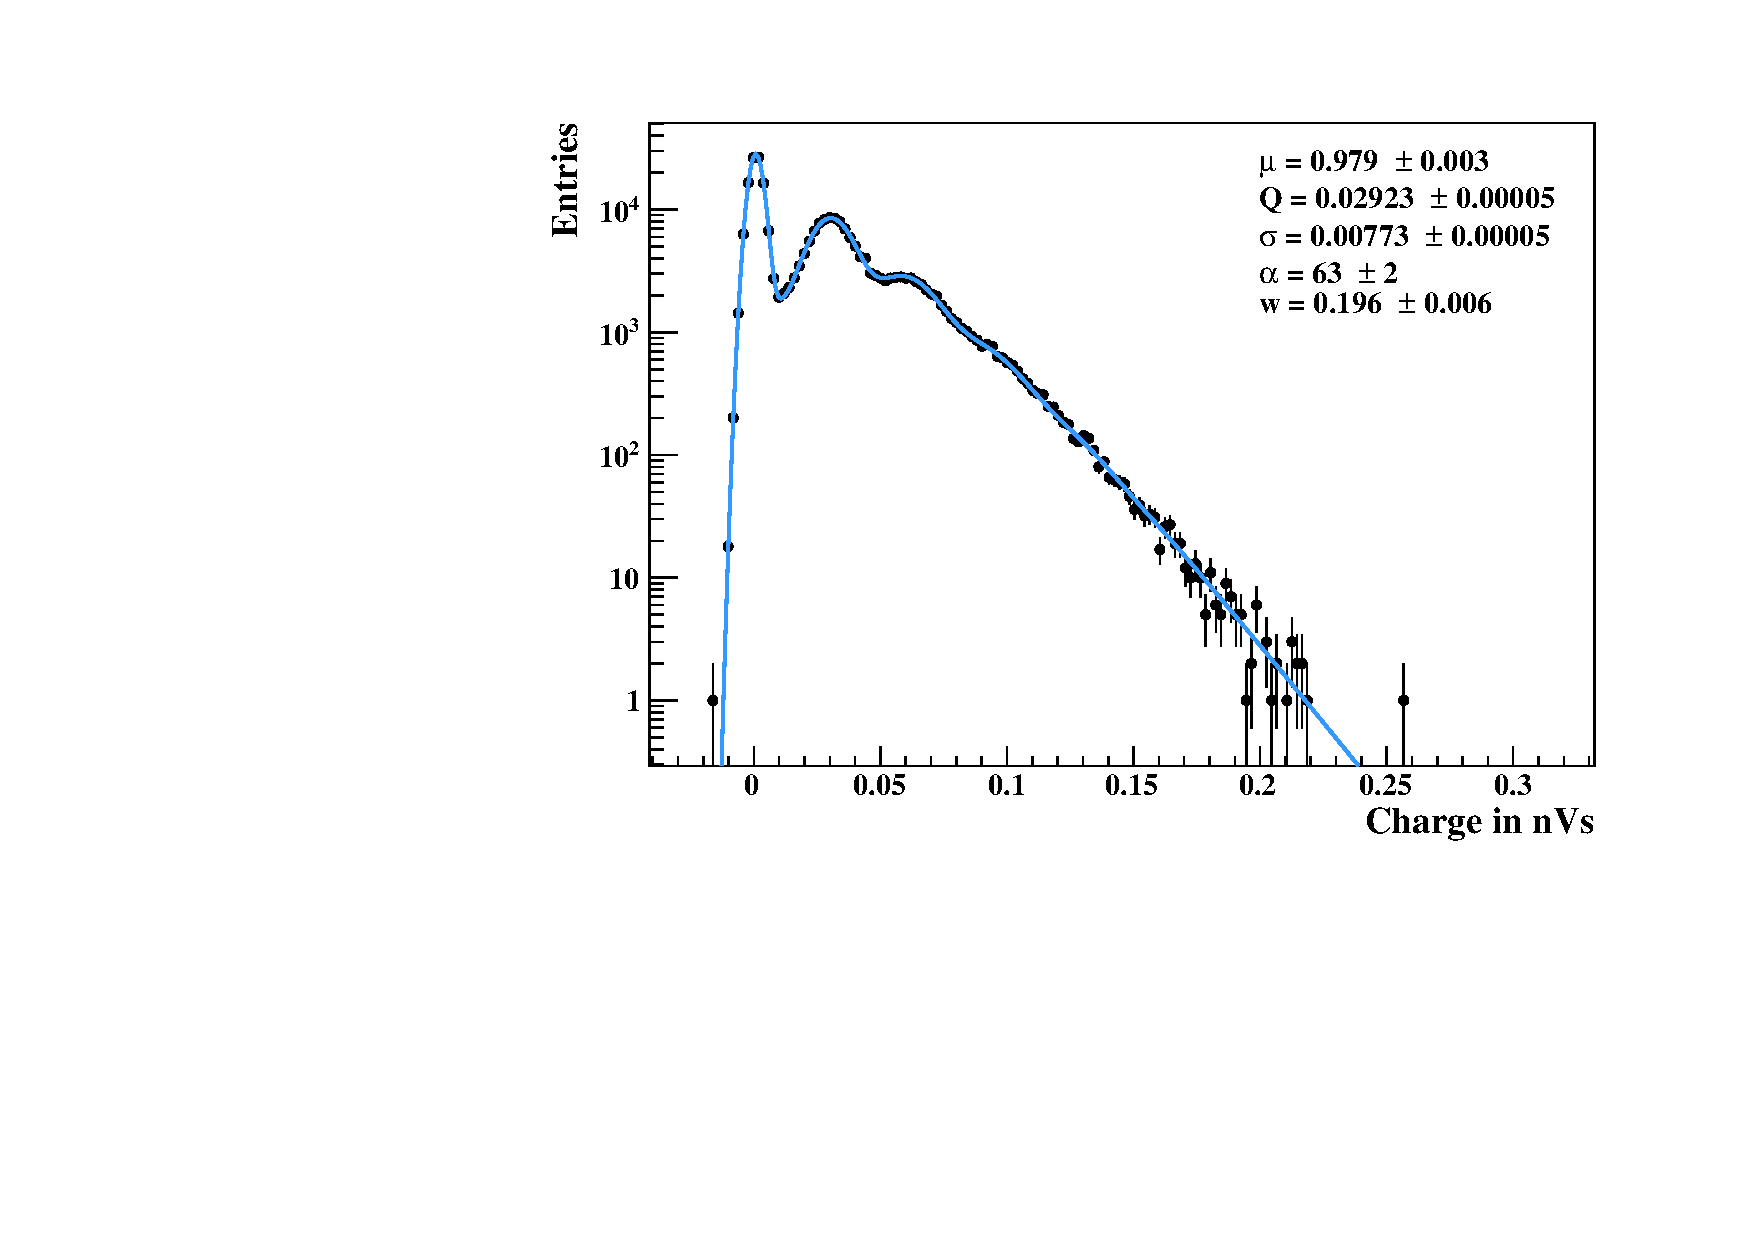
\includegraphics[width=11.3cm, height=7.8cm]{figures/fit-3.pdf} %\\
\caption{A few fits obtained using the analytical model of $S_R(x)$.  The data are shown in the black dots and the best fit curve is shown in azure line. }
\label{fig:spe}
\end{figure}
Figure~\ref{fig:spe} shows examples of two SPE charge distributions obtained through this procedure. 
The chain followed by the analysis has been described before and it will not be repeated here as well.\footnote{See ref.~\cite{me2} for more details.} 
We only note that the multidimensional fit of $S_R(x)$ is quite complicated and it is likely to fail unless good initial values and limits are set to the fitting parameters.  
One can easily see, in figure~\ref{fig:spe}, that the best fit curve (azure line) follows closely the data points and that the model reproduces the experimental measurements. 
In all cases the $\chi^2$/NDOF was close to one. 
Table~\ref{tab:g} shows the gain obtained through the DFT method~\cite{me} and the analytical model. 
We remind the reader that the gain $Q_s$ is given by:
\begin{align}
Q_s  = \frac{w}{\alpha} + (1-w)Q_g. 
\end{align}
The first row shows the Poisson mean $\mu$ extracted by the fitter for reference purposes. 
One can observe that as $\mu$ increases the gain remains quite stable and the results between the DFT and the analytical model are almost identical. 
We should also note that a drift in the gain is observed, but this is too small in magnitude.   

\begin{table}[t!]
\centering
\begin{tabular}{| c  || c | c |}
\hline
$\mu$                      & Gain from the DFT method  	       & Gain from the analytical model           \\[0.6ex] \hline\hline
0.543 $\pm$ 0.003  & 0.02620					       & 0.02619 						     				\\
0.632 $\pm$ 0.003  & 0.02646					       & 0.02645					  	    				\\
0.768 $\pm$ 0.003  & 0.02649					       & 0.02648					  	    				\\
0.979 $\pm$ 0.003  & 0.02660					       & 0.02659					    	    				\\
1.357 $\pm$ 0.005  & 0.02681					       & 0.02681					  	    				\\
2.014 $\pm$ 0.008  & 0.02682					       & 0.02682				  			
\\[0.6ex] \hline\hline
\end{tabular}
\caption{Summary of the R7081 PMT calibration results.}
\label{tab:g}
\end{table}



\section{Outlook}
\label{sec:outro}
%
In this article we have a have presented an analytical model that can be used for the calibration of PMTs whenever the SPE response can be parameterized by eq.~\ref{eq:S}.  
The various mathematical formulae were derived with great detail and attention was paid to showcase the approximations needed for the final solution. 
We should emphasize that while the equations might seem, at first glance, both complicated and unnecessarily elaborate we find that the model is quite simple 
and that it can be employed with the same efficacy as the already establish approaches. 
Data from a R7081 PMT were analyzed and the results were in excellent agreement with those obtained using the DFT method. 
In particular, the gain parameter of the PMT was remarkably stable within the $\mu$~$\sim$~0.5 - 2.0 plateau. 
The code used for these investigations exists in a public repository~\cite{git}.  




%\newpage
\appendix
%

\section{$\int_{ x_1 }^{x_2}  e^{-a x^2 +b x +c } \ dx$ integral}
\label{app:int}
%

The integral, 
\begin{align}
I = \int_{ x_1 }^{x_2}  e^{-a x^2 +b x +c } \ dx,
\end{align}
occurs frequently in calculations involving $S_R(x)$ functions with SPE responses parameterized with gaussians, and so we think that it is rather instructive to derive its formula in this appendix. 
\begin{align}
I = & \int_{ x_1 }^{x_2}  e^{-a x^2 +b x +c } \ dx \nonumber \\
  = & e^c \int_{ x_1 }^{x_2}  e^{-a ( x^2 - \frac{b}{a} x )} \ dx  \nonumber \\
  = & e^{\frac{b^2}{4a}+c} \int_{ x_1 }^{x_2}  e^{-a ( x - \frac{b}{2a} )^2} \ dx. 
\end{align}
Using the substitution: 
\begin{align}
u = \sqrt{a} ( x - \frac{b}{2a} )  
\end{align}
$I$ becomes,
\begin{align}
I = &  \frac{1}{\sqrt{a}} e^{\frac{b^2}{4a}+c} \int_{ \frac{2a x_1 -b }{2\sqrt{a}} }^{ \frac{2a x_2 -b }{2\sqrt{a}} }  e^{-u^2 } \ du \nonumber \\
  = & \frac{1}{\sqrt{a}} e^{\frac{b^2}{4a}+c} \left(   \int_{ 0 }^{ \frac{2a x_2 -b }{2\sqrt{a}} }  e^{-u^2 } \ du -  \int^{ \frac{2a x_1 -b }{2\sqrt{a}} }_{ 0 }  e^{-u^2 } \ du\right)  \nonumber \\
  = &  \frac{1}{2}  \sqrt{\frac{\pi}{a} } e^{\frac{b^2}{4a}+c} \left[ \text{erf}\left({ \frac{2a x -b }{2\sqrt{a}} }\right) \right]^{ x_2 }_{ x_1 }.
\end{align}
In the last line we made use of the definition:
\begin{align}
 \text{erf}(x) = \frac{2}{\sqrt{\pi}} \int_0^x e^{-t^2} dt. 
 \end{align}
 Now, if $x_2\rightarrow +\infty$ the integral simplifies to:
 \begin{align}
I = &  \frac{1}{2}  \sqrt{\frac{\pi}{a} } e^{\frac{b^2}{4a}+c} \left( 1 - \text{erf}\left({ \frac{2a x_1 -b }{2\sqrt{a}} }\right) \right) \nonumber \\
  = & \frac{1}{2}  \sqrt{\frac{\pi}{a} } \ e^{\frac{b^2}{4a}+c} \ \text{erfc}\left({ \frac{2a x_1 -b }{2\sqrt{a}} }\right). \label{eq:intg}
\end{align}


\section{Formulae for $(f*B)(x)$ and $(g*B)(x)$}
\label{app:sr1}
%

\subsection*{Case of $(f*B)(x)$ }
%

We start with a direct calculation of the $(f*B)(x)$ convolution integral:
\begin{align}
(f*B)(x) = & \frac{\alpha}{\sqrt{2\pi}\sigma_0}   \int^{+\infty}_{-\infty} e^{ -\frac{(x-Q_0-t)^2}{2\sigma_0^2} -\alpha t } H(t) dt \nonumber \\
             = & \frac{\alpha}{\sqrt{2\pi}\sigma_0}  \int^{+\infty}_{0} e^{ -\frac{(x-Q_0-t)^2}{2\sigma_0^2} -\alpha t } dt.
\end{align}
Through the substitution:
\begin{align}
u = \frac{t+Q_0-x}{\sqrt{2}\sigma_0}  
\end{align}
the expression becomes:
\begin{align}
(f*B)(x) = & \frac{\alpha }{\sqrt{\pi}}   \int^{+\infty}_{ \frac{Q_0-x}{\sqrt{2}\sigma_0}   } e^{ -u^2 -\alpha( \sqrt{2}\sigma_0 u + x - Q_0 ) } dt \nonumber \\
            = & \frac{\alpha }{\sqrt{\pi}} e^{-\alpha(x-Q_0)} \int^{+\infty}_{ \frac{Q_0-x}{\sqrt{2}\sigma_0}   } e^{ -u^2 - \sqrt{2}\alpha\sigma_0 u  } dt  \nonumber \\
            = & \frac{\alpha }{2} e^{\frac{\alpha^2\sigma_0^2}{2}} e^{-\alpha(x-Q)} \ \text{erfc}\left(    \frac{Q_0 + \alpha\sigma_0^2 -x }{\sqrt{2}\sigma_0} \right).
\end{align}
In the last line we employed the integral identity~\eqref{eq:intg}. 


\subsection*{Case of $(g*B)(x)$ }
%

In a similar way the calculation of  $(g*B)(x)$ proceeds. 
\begin{align}
(g*B)(x) = & \frac{1 }{g_N}  \frac{1 }{\sqrt{2\pi}\sigma} \frac{1 }{\sqrt{2\pi}\sigma_0} \int^{+\infty}_{ -\infty  }  e^{-\frac{(t-Q)^2}{2\sigma^2} - \frac{(x-t-Q_0)^2}{2\sigma_0^2}} H(t) dt
\end{align}
\begin{align}
I = & \int^{+\infty}_{ -\infty  }  e^{-\frac{(t-Q)^2}{2\sigma^2} - \frac{(x-t-Q_0)^2}{2\sigma_0^2}} H(t) dt \nonumber \\
  = & \int^{+\infty}_{ 0  }  e^{-\frac{(t-Q)^2}{2\sigma^2} - \frac{(x-t-Q_0)^2}{2\sigma_0^2}} dt
\end{align}
With the substitutions,
\begin{align}
u = \frac{t-Q}{\sigma} \ \  \text{and}\  \ Q^\prime = x - Q - Q_0,
\end{align}
$I$ takes the form:
\begin{align}
I = \ & \sigma \int^{+\infty}_{ -\frac{Q}{\sigma}  }  e^{-\frac{u^2}{2} - \frac{(Q^\prime-\sigma u )^2}{2\sigma_0^2}} du \nonumber \\
  = \ & \sigma \int^{+\infty}_{ -\frac{Q}{\sigma}  } e^{-\frac{\sigma^2+\sigma_0^2}{2\sigma_0^2 }u^2 + \frac{Q^\prime\sigma}{\sigma_0^2}u - \frac{Q^{\prime 2}}{2\sigma_0^2}  } du \nonumber \\
  %= \ & \frac{1}{2} \sqrt{2\pi} \sigma \sigma_0 \frac{1}{\sqrt{\sigma^2 +\sigma_0^2}} \ e^{-\frac{Q^{\prime2} }{2(\sigma^2+\sigma_0^2)}} 
  %\text{erfc} 
  %\left(    \frac{ Q_0\sigma^2 -Q\sigma_0^2 -x \sigma^2  }{\sqrt{2} \sigma_0\sigma\sqrt{\sigma_0^2 + \sigma^2} }         \right) \nonumber \\  
  = \ &  \frac{1}{2} \sqrt{2\pi} \sigma \sigma_0 \frac{1}{\sqrt{\sigma^2 +\sigma_0^2}} \ e^{ -\frac{(x-Q_0-Q)^2}{2( \sigma_0^2 + \sigma^2 )}} 
  \text{erfc} 
  \left(    \frac{ Q_0\sigma^2 -Q\sigma_0^2 -x \sigma^2  }{\sqrt{2} \sigma_0\sigma\sqrt{\sigma_0^2 + \sigma^2} }         \right). 
\end{align}
Again we made use of the integral of appendix~\ref{app:int}. 
Plugging $I$ into the initial equation for $(g*B)(x)$ we are left with the solution: 
\begin{align}
(g*B)(x) = \frac{1}{2} \frac{1}{\sqrt{2\pi}} \frac{1}{\sqrt{\sigma^2 +\sigma_0^2}}  \frac{1}{g_N} \ e^{ -\frac{(x-Q_0-Q)^2}{2( \sigma_0^2 + \sigma^2 )}} 
\text{erfc} 
  \left(    \frac{ Q_0\sigma^2 -Q\sigma_0^2 -x \sigma^2  }{\sqrt{2} \sigma_0\sigma\sqrt{\sigma_0^2 + \sigma^2} }         \right). 
\end{align}

\section{Calculation of $h_{m,n}(x)$}
%The $I_{m,n}$ integral}
\label{app:Imn}
%

We first write down the formula for $f_m(x)$:
\begin{align}
f_m(x) =  \frac{\alpha (\alpha x )^{m-1}}{(m-1)!} e^{-\alpha x } H(x),
\end{align}
which one can easily prove by induction. 
$h_{m,n}(x)$ becomes:
\begin{align}
h_{m,n}(x) = & \frac{ \alpha^{m}}{(m-1)!} \frac{1}{\sqrt{2\pi}\sigma_{n-m}} \int_{-\infty}^{+\infty} t^{m-1} e^{ -\frac{ (x-t -Q_{n-m})^2}{2\sigma^2_{n-m}}-\alpha t} H(t) dt \nonumber \\
                  = & \frac{ \alpha^{m}}{(m-1)!} \frac{1}{\sqrt{2\pi}\sigma_{n-m}} \int_{0}^{+\infty} t^{m-1} e^{ -\frac{ (x-t -Q_{n-m})^2}{2\sigma^2_{n-m}}-\alpha t} dt.
\end{align}
Note that $G_{n-m}(x)$ was replaced with a symmetric gaussian. 
Completing the square in the exponential one has:
\begin{align}
h_{m,n}(x) = & \frac{ \alpha^{m}}{(m-1)!} \frac{1}{\sqrt{2\pi}\sigma_{n-m}} \int_{0}^{+\infty} t^{m-1} e^{  \omega^2  -\psi^2  -\left( \frac{t}{\sqrt{2}\sigma_{n-m}} - \omega \right)^2} dt,
\end{align}
with 
\begin{align}
\psi = & \frac{x-Q_{n-m}}{\sqrt{2}\sigma_{n-m}}, \\
\omega = & \frac{x-Q_{n-m} -\lambda\sigma^2_{n-m}}{\sqrt{2}\sigma_{n-m}}.
\end{align}  
The integral:
\begin{align}
I =  e^{  \omega^2  -\psi^2 }\int_{0}^{+\infty} t^{m-1} e^{  -\left( \frac{t}{\sqrt{2}\sigma_{n-m}} - \omega \right)^2} dt,
\end{align}
becomes with the substitution:
\begin{align}
u = \frac{t}{\sqrt{2}\sigma_{n-m}},
\end{align}
\begin{align}
I =  (\sqrt{2}\sigma_{n-m})^m e^{  \omega^2  -\psi^2 }\int_{0}^{+\infty} u^{m-1} e^{  -\left( u - \omega \right)^2} du.
\end{align}
Now, the integral:
\begin{align}
I^\prime = \int_{0}^{+\infty} u^{m-1} e^{  -\left( u - \omega \right)^2} du,
\end{align}
was solved using the \emph{Mathematica} online software~\cite{math} and the result is:
\begin{align}
I^\prime = \frac{1}{2} e^{-\omega^2} 
\left(\  \Gamma\left( \frac{m}{2} \right) M\left( \frac{m}{2}, \frac{1}{2}, \omega^2 \right)  + 2\omega \Gamma\left( \frac{m+1}{2} \right) M\left(\frac{m+1}{2}, \frac{3}{2}, \omega^2  \right) \ \right).  
\end{align}
Finally, and using the formulae for $I$ and $I^\prime$, $h_{m,n}(x)$ takes the form:
\begin{align}
h_{m,n}(x) =  \frac{ \alpha (\alpha\sqrt{2} \sigma_{n-m})^{m-1}}{(m-1)!} \frac{1}{2\sqrt{\pi}} \  I_{m,n}
\end{align} 
where $I_{m,n}$  is given by the equation:
\begin{align}
I_{m,n} = e^{-\psi^2} \left(\  \ \Gamma\left( \frac{m}{2} \right) M\left( \frac{m}{2}, \frac{1}{2}, \omega^2 \right)  + 2\omega \Gamma\left( \frac{m+1}{2} \right) M\left(\frac{m+1}{2}, \frac{3}{2}, \omega^2 \ \right) \ \right).  
\end{align}

\subsection*{$I_{m,n}$ case I: $\omega> 0$ and $\omega^2 \gg 0$ }
%

We first treat the case where $\omega$ is positive and $\omega^2$ is far greater than zero, $\omega^2 \gg 0$.  
We take advantage of the asymptotic formula for $M(a,b,z)$ when $z \gg 0$:
\begin{align}
M(a,b,z) = \frac{\Gamma (b)}{\Gamma(a)} \  e^z z^{a-b}.
\end{align}
We then have for $I_{m,n}$:
\begin{align}
 I_{m,n} = 2\sqrt{\pi}   e^{\omega^2 - \psi^2 + (m-1) \ell n |\omega|}.
\end{align}

\subsection*{$I_{m,n}$ case II: $\omega >0$}
%

We use Kummer's transformation:
\begin{align}
M(a,b,z) = e^z M(b-a,b,-z)
\end{align}
and $I_{m,n}$ becomes:
\begin{align}
I_{m,n} = e^{\omega^2 -\psi^2 } \left(\  \Gamma\left( \frac{m}{2} \right) M\left(-\frac{m-1}{2}, \frac{1}{2}, -\omega^2 \right)  + 2|\omega| \Gamma\left( \frac{m+1}{2} \right) M\left(1-\frac{m}{2}, \frac{3}{2}, -\omega^2 \right)   \    \right).
\end{align}

\subsection*{$I_{m,n}$ case III: $ \omega <0$}
%

For negative values of $\omega$ one can exploit the relation:
\begin{align}
U(a,b,z) = \frac{\Gamma(1-b) }{\Gamma(a+1-b)}M(a,b,z) + \frac{\Gamma(b-1) }{\Gamma(a)} z^{1-b} M(a+1-b, 2-b, z )
\end{align}
and write $I_{m,n}$ as:
\begin{align}
I_{m,n} = e^{ -\psi^2 } \Gamma\left( \frac{m}{2} \right)   \Gamma\left( \frac{m+1}{2} \right) \frac{1}{\sqrt{\pi}} U\left( \frac{m}{2}, \frac{1}{2}, \omega^2  \right). 
\end{align}
We note that a similar  asymptotic relation for $U(a,b,z)$ can be written for $\omega<0$ and $\omega^2 \gg 0$. 


\acknowledgments
%

The data used in this publication were taken in the laboratory of M. Dracos and we wish to thank him for allowing us to use them for the purposes of this communication. 
We also wish to thank C.~Bobeth for encouraging us to continue and complete this study.

%\paragraph{Note added.} This is also a good position for notes added
%after the paper has been written.

% We suggest to always provide author, title and journal data:
% in short all the informations that clearly identify a document.

\begin{thebibliography}{99}

\bibitem{bellamy} E. H. Bellamy {et al.}, \emph{Absolute Calibration and Monitoring of a spectrometric channel using a photomultiplier}, 
\href{https://www.sciencedirect.com/science/article/pii/016890029490183X}{\emph{Nucl. Instrum. Meth.} {\bf A 339} (1994) 468-476}. 

\bibitem{dossi}  R. Dossi {et al.}, \emph{Methods for precise photoelectron counting with photomultipliers}, 
\href{https://www.sciencedirect.com/science/article/pii/S0168900200003375}{\emph{Nucl. Instrum. Meth.} {\bf A 451} (2000) 623-637}.

\bibitem{darkside} T. Alexander {et al.} (DarkSide Collaboration), \emph{Light Yield in DarkSide-10: a Prototype Two-phase Argon TPC for Dark Matter Searches}, 
\href{https://www.sciencedirect.com/science/article/pii/S0927650513001254?via\%3Dihub}{\emph{Astropart. Phys.} {\bf 49} (2013) 44-51}.
%[\href{https://arxiv.org/abs/1204.6218}{\texttt{arXiv:1204.6218}}]. 

\bibitem{me2} L. N. Kalousis {et al.}, \emph{A fast numerical method for photomultiplier calibration},\\  
\href{https://iopscience.iop.org/article/10.1088/1748-0221/15/03/P03023}{\emph{JINST} {\bf 15} (2020) P03023}.

\bibitem{binom} \href{https://en.wikipedia.org/wiki/Binomial_theorem}{https://en.wikipedia.org/wiki/Binomial\_theorem}

\bibitem{erf} \href{https://en.wikipedia.org/wiki/Error_function}{https://en.wikipedia.org/wiki/Error\_function}

\bibitem{me} L. N. Kalousis {et al.}, \emph{Calibration of the Hamamatsu R7081 photomultiplier tube}, \\ \emph{submitted to JINST} 
[\href{https://arxiv.org/abs/2304.07292}{\texttt{arXiv:2304.07292}}]. 

\bibitem{git} \href{https://github.com/kalousis/PMTCalib}{https://github.com/lkalousis/PMTCalib}

\bibitem{math} Wolfram Research, Inc. (\href{www.wolfram.com}{www.wolfram.com}), Mathematica Online, Champaign, IL (2022).

\end{thebibliography}
\end{document}
